\documentclass[a4paper,12pt]{article}
\usepackage{ctex}
\usepackage{amsmath}
\usepackage{amssymb}
\usepackage{graphicx}
\usepackage{float}
\usepackage{geometry}
\geometry{left=2.5cm,right=2.5cm,top=2.5cm,bottom=2.5cm}

\title{\textbf{计算机辅助几何设计 - 作业 10}}
\author{刘行 \\ 学号: PB22000150}
\date{\today}

\begin{document}

\maketitle

\section{实验目的}

本次作业的主要目的是实现三角网格的参数化算法,将 3D 曲面映射到 2D 平面上。具体要求是基于 Floater (1997) 的算法,使用保形权重(Shape-Preserving Weights)完成 Tutte Embedding。实验对象为提供的 \texttt{cathead.obj} 模型,需要在 \texttt{tutte\_test.m} 框架下完成核心函数的编写。

\section{实验原理}

\subsection{Tutte Embedding}
Tutte 嵌入定理指出,对于一个 3-连通平面图,如果将其边界顶点映射到一个凸多边形上,并将所有内部顶点放置在其邻居的加权中心位置,则该图的直线嵌入是平面性的(即没有边交叉)。
对于内部顶点 $i$,其位置 $\mathbf{y}_i$ 满足:
\begin{equation}
    \mathbf{y}_i = \sum_{j \in N(i)} \lambda_{ij} \mathbf{y}_j, \quad \text{其中} \sum_{j \in N(i)} \lambda_{ij} = 1
\end{equation}
这转化为求解线性方程组 $L\mathbf{y} = \mathbf{b}$,其中 $L$ 为拉普拉斯矩阵。

\subsection{保形权重 (Floater 算法)}
为了尽可能保持网格的几何形状,减少参数化过程中的角度变形,我们不使用统一权重,而是采用**距离倒数权重**(Inverse Distance Weights)。对于边 $(i, j)$,其权重 $w_{ij}$ 计算公式为:
\begin{equation}
    w_{ij} = \frac{1}{\|\mathbf{x}_i - \mathbf{x}_j\|}
\end{equation}
其中 $\|\mathbf{x}_i - \mathbf{x}_j\|$ 为 3D 空间中的欧几里得距离。相比于统一权重,这种方法更能反映原始网格的几何特征。

\section{算法逻辑与实现步骤}

在 \texttt{tutte\_embed} 函数中,算法的具体实现逻辑如下:

\begin{enumerate}
    \item \textbf{边界识别与提取}:
    首先,利用提供的辅助函数 \texttt{findBoundary} 提取网格的边界顶点索引序列。这是参数化的基础,因为边界需要被固定。
    
    \item \textbf{边界映射(凸组合条件)}:
    为了满足 Tutte 定理的凸边界条件,我们将提取出的边界顶点映射到 2D 平面的单位圆上。通过将角度区间 $[0, 2\pi]$ 均匀分割,计算出每个边界顶点对应的 $(\cos\theta, \sin\theta)$ 坐标。
    
    \item \textbf{构建权重矩阵}:
    遍历网格的所有边。对于每一条边,计算其在 3D 空间中的长度,并取长度的倒数作为权重 $w$。如果是统一权重(Uniform),则权重设为 1;但在本实验中,为了保形,我们严格执行距离倒数计算。
    
    \item \textbf{构建拉普拉斯系统}:
    基于计算出的权重构建稀疏矩阵 $W$。接着计算度矩阵 $D$($W$ 的行和),进而得到拉普拉斯矩阵 $L = D - W$。
    
    \item \textbf{施加边界条件并求解}:
    这是一个带有狄利克雷边界条件(Dirichlet Boundary Condition)的线性系统。我们将矩阵 $L$ 中对应边界顶点的行替换为单位矩阵的行(即对角线元素设为 1,其余为 0),并将方程右端项(RHS)中对应的位置设为之前计算好的单位圆坐标。最后,使用 MATLAB 的左除运算符求解稀疏线性方程组 $L\mathbf{y} = \text{RHS}$,得到所有顶点的 2D 坐标。
\end{enumerate}

\section{实验结果与分析}

实验使用 \texttt{readObj} 读取模型,并调用实现的算法进行测试。

\begin{figure}[H]
    \centering
    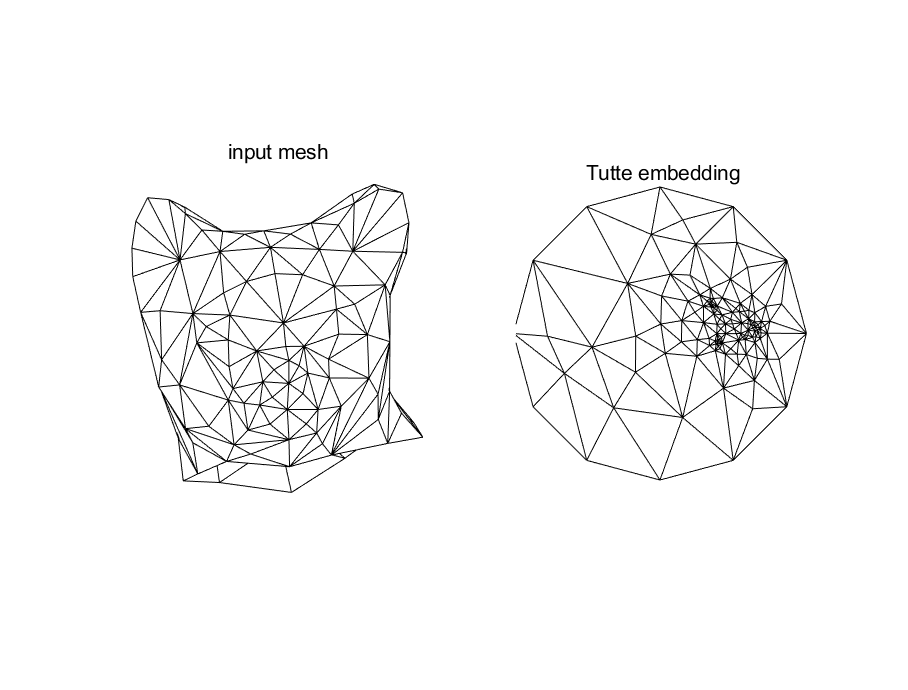
\includegraphics[width=0.5\textwidth]{fig/result.eps}
    \caption{实验结果对比:左图为原始 3D 网格 (Input Mesh),右图为 Tutte 参数化结果 (Embedding)。}
    \label{fig:result}
\end{figure}

如图 \ref{fig:result} 所示,左侧展示了原始的 \texttt{cathead} 模型,具有复杂的曲面几何特征。右侧展示了经过 Tutte Embedding 算法处理后的参数化结果。

观察结果可以得出:
\begin{itemize}
    \item \textbf{边界映射}:网格边界被成功映射为了一个标准的凸多边形(圆形),符合算法预期。
    \item \textbf{拓扑结构}:内部网格线没有发生折叠或交叉,证明了生成的是有效的平面三角剖分。
    \item \textbf{形状保持}:由于使用了距离倒数权重,参数化后的网格密度分布在一定程度上反映了原模型的几何特征,相比于统一权重的参数化,这种方法通常能产生更平滑的过渡。
\end{itemize}

\end{document}